\documentclass[a4paper]{article}
\usepackage[utf8]{inputenc}
\usepackage{alphabeta}
\usepackage{graphicx}
\usepackage[section]{placeins}
\usepackage{float}
\usepackage{amsmath}
\usepackage{listings}
\usepackage{xcolor}
\usepackage{amsmath}
\usepackage{extarrows}
\usepackage{amssymb}
\usepackage{verbatim}
\usepackage{enumerate}
\usepackage{eurosym}
\usepackage{svg}
\usepackage{varwidth}

\definecolor{codegreen}{rgb}{0,0.6,0}
\definecolor{codegray}{rgb}{0.5,0.5,0.5}
\definecolor{codepurple}{rgb}{0.58,0,0.82}
\definecolor{backcolour}{rgb}{0.95,0.95,0.92}

\lstdefinestyle{mystyle}{
    backgroundcolor=\color{backcolour},   
    commentstyle=\color{codegreen},
    keywordstyle=\color{magenta},
    numberstyle=\tiny\color{codegray},
    stringstyle=\color{codepurple},
    basicstyle=\ttfamily\footnotesize,
    breakatwhitespace=false,         
    breaklines=true,                 
    captionpos=b,                    
    keepspaces=true,                 
    numbers=left,                    
    numbersep=5pt,                  
    showspaces=false,                
    showstringspaces=false,
    showtabs=false,                  
    tabsize=2
}

\lstset{style=mystyle}

\setlength{\parindent}{0pt}
\setlength{\parskip}{1em}
\setlength{\jot}{4mm}

\title{Συστήματα Αναμονής \\ 2η εργαστηριακή άσκηση}
\author{Νικόλαος Παγώνας, el18175}
\date{}

\begin{document}

\maketitle

\subsection*{Θεωρητική μελέτη της ουράς Μ/Μ/1}

\subsubsection*{(α)} Προκειμένου να είναι εργοδική η ουρά Μ/Μ/1, είναι απαραίτητο να ισχύει $ {ρ = \dfrac{λ}{μ} < 1} $, όπου $ λ $ ο ρυθμός αφίξεων, $ μ $ ο ρυθμός εξυπηρέτησης και $ ρ $ η ένταση φορτίου.

Σχεδιάζουμε το διάγραμμα ρυθμού μεταβάσεων για την ουρά Μ/Μ/1:

\begin{center}
	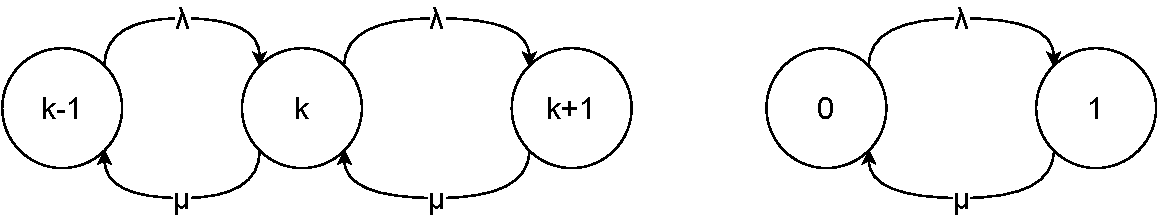
\includegraphics[width=\textwidth]{files/1a.pdf} 
\end{center}

Για τον υπολογισμό των εργοδικών πιθανοτήτων των καταστάσεων του συστήματος από τις εξισώσεις ισορροπίας έχουμε:

\[
	(λ+μ)P_k=λP_{k-1}+μP_{k+1} \text{  για  } k \geq 1 \text{  και  } λP_0=μP_1 
\]

οπότε από την δεύτερη εξίσωση  παίρνουμε:
\[
	P_1=\left(\frac{λ}{μ}\right)P_0 = ρP_0
\]

Αντικαθιστώντας στην πρώτη (για $k=1$) έχουμε:
\[
	(λ+μ)P_1=λP_0+μP_2 \implies P_2=\frac{λ}{μ}P_1=\left(\frac{λ}{μ}\right)^2P_0 = ρ^2P_0
\]

και γενικά:

\[
	P_k = ρ^kP_0, \ \ k>0 
\]

Επειδή επιπλέον ισχύει η ιδιότητα της κανονικοποίησης:

\[
	\sum_{k=0}^\infty P_k = 1 \implies 
	\sum_{k=0}^\infty ρ^kP_0=1 \implies
	P_0\cdot\frac{1}{1-ρ} = 1 \text{ (αφού } ρ < 1)
\] 

και έτσι:

\[
	P_0 = 1-ρ, \ P_k = (1-ρ)ρ^k, \text{ για } k > 0
\]

\subsubsection*{(β)}

Θεωρούμε γνωστή την ισότητα της εκφώνησης (έχει αποδειχθεί και στο μάθημα) και χρησιμοποιούμε τον νόμο του Little:

\[
	E[T]=\frac{E[n(t)]}{γ} = \frac{E[n(t)]}{λ} = \frac{ρ}{(1-ρ)λ} = \frac{λ/μ}{λ(1-λ/μ)} = \frac{1}{μ-λ}
\]
\subsubsection*{(γ)}

Η ουρά Μ/Μ/1 χαρακτηρίζεται από άπειρη χωρητικότητα και απείρως επισκέψιμες επαναληπτικές καταστάσεις (positive recurrent states), με μη μηδενικές εργοδικές πιθανότητες $ P_k(t) \to P_k > 0, \ k=0,1,2,...$ 

Αυτό σημαίνει ότι (σε άπειρο χρόνο) θα συναντήσουμε όλες τις καταστάσεις, και από άπειρες φορές. Επομένως, αφού η κατάσταση 57 ανήκει στην απειρία αυτή, τότε θα υπάρξει χρονική στιγμή που το σύστημα θα βρεθεί με 57 πελάτες.

\subsection*{Ανάλυση ουράς Μ/Μ/1 με Octave}

\subsubsection*{(α)}

Προκειμένου το σύστημα να είναι εργοδικό, θα πρέπει: 
\[ 
	ρ = λ/μ < 1 \implies μ > λ \implies μ > 5 \ \frac{\text{πελάτες}}{\text{min}}
\]
\subsubsection*{(β)}

Με τη βοήθεια της συνάρτησης qsmm1 του πακέτου queueing του Octave απεικονίζουμε τα παρακάτω 4 διαγράμματα, για τις επιτρεπόμενες τιμές του $ μ, \text{ δηλαδή } μ \in(5,10]$:

\begin{minipage}{\textwidth}
	1. Βαθμός χρησιμοποίησης (utilization) ως προς το ρυθμό εξυπηρέτησης:
	\[
		u = \frac{γ}{μ} = \frac{λ}{μ}
	\]	
	\begin{figure}[H]
		\begin{center}
			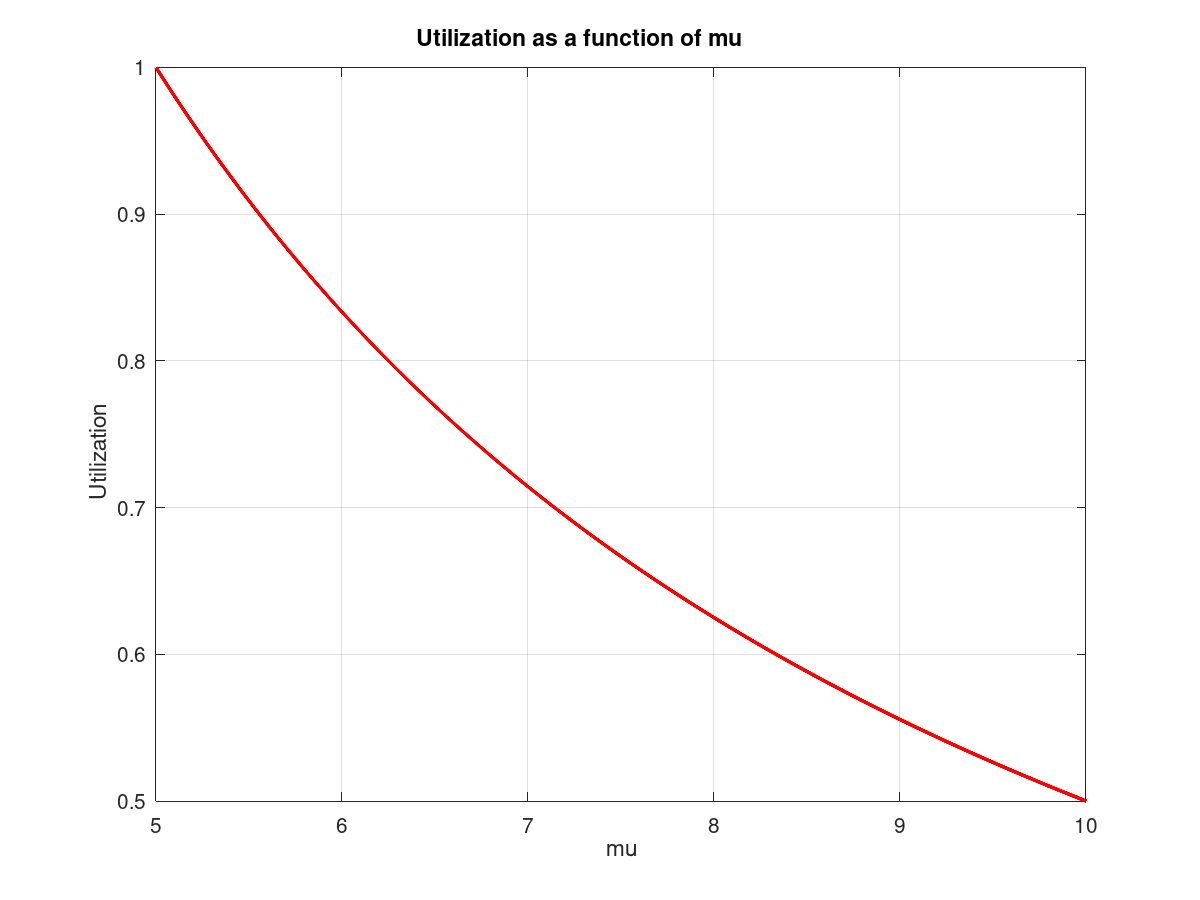
\includegraphics[width=0.85\textwidth]{files/2b1.png}
		\end{center}
	\end{figure}
\end{minipage}

\begin{minipage}{\textwidth}
	2. Μέσος χρόνος καθυστέρησης του συστήματος E[T] ως προς το ρυθμό εξυπηρέτησης:
	\[
		E[T] = \frac{1}{μ-λ}
	\]
	\begin{figure}[H]
		\begin{center}
			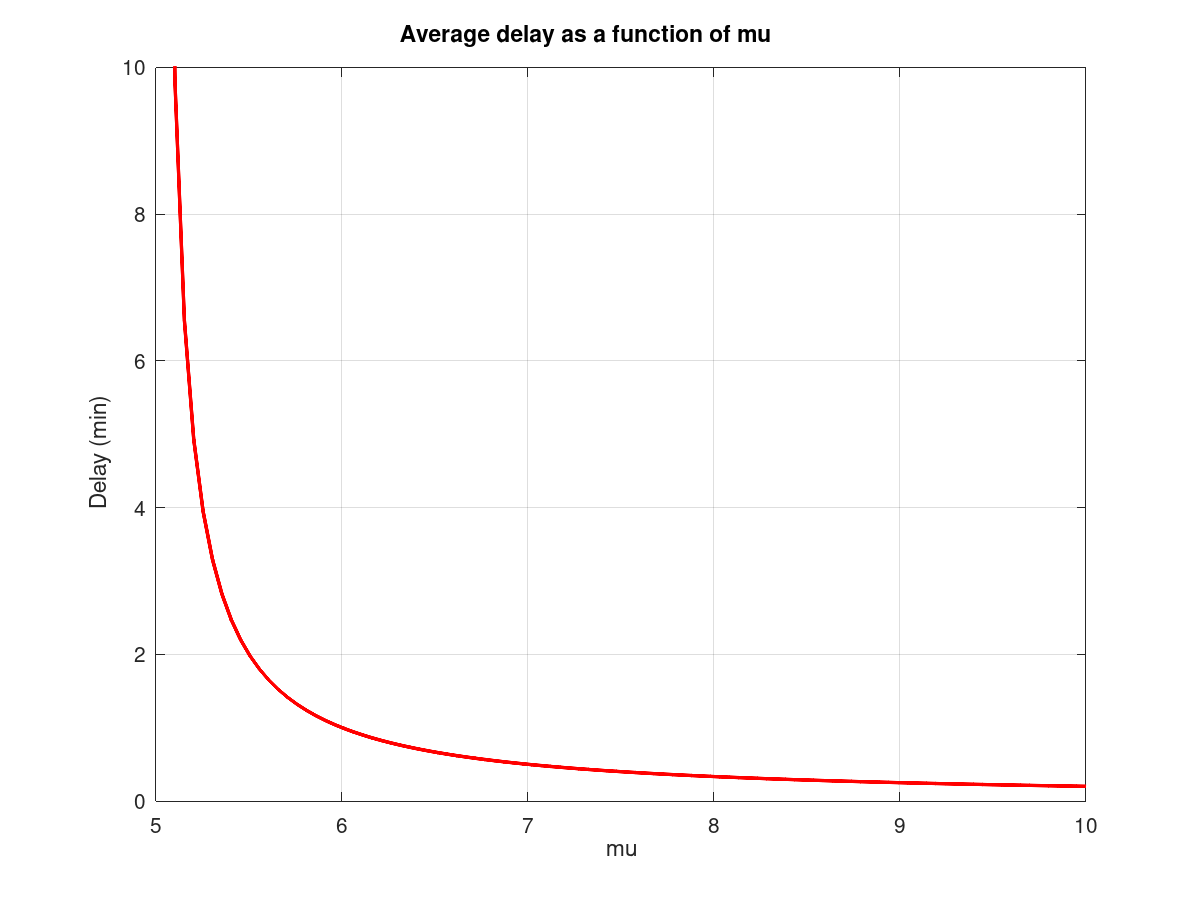
\includegraphics[width=0.85\textwidth]{files/2b2.png}
		\end{center}
	\end{figure}
\end{minipage}

\begin{minipage}{\textwidth}
	3. Μέσος αριθμός πελατών στο σύστημα ως προς το ρυθμό εξυπηρέτησης:
	\[
		E[n(t)] = \frac{ρ}{1-ρ}
	\]
	\begin{figure}[H]
		\begin{center}
			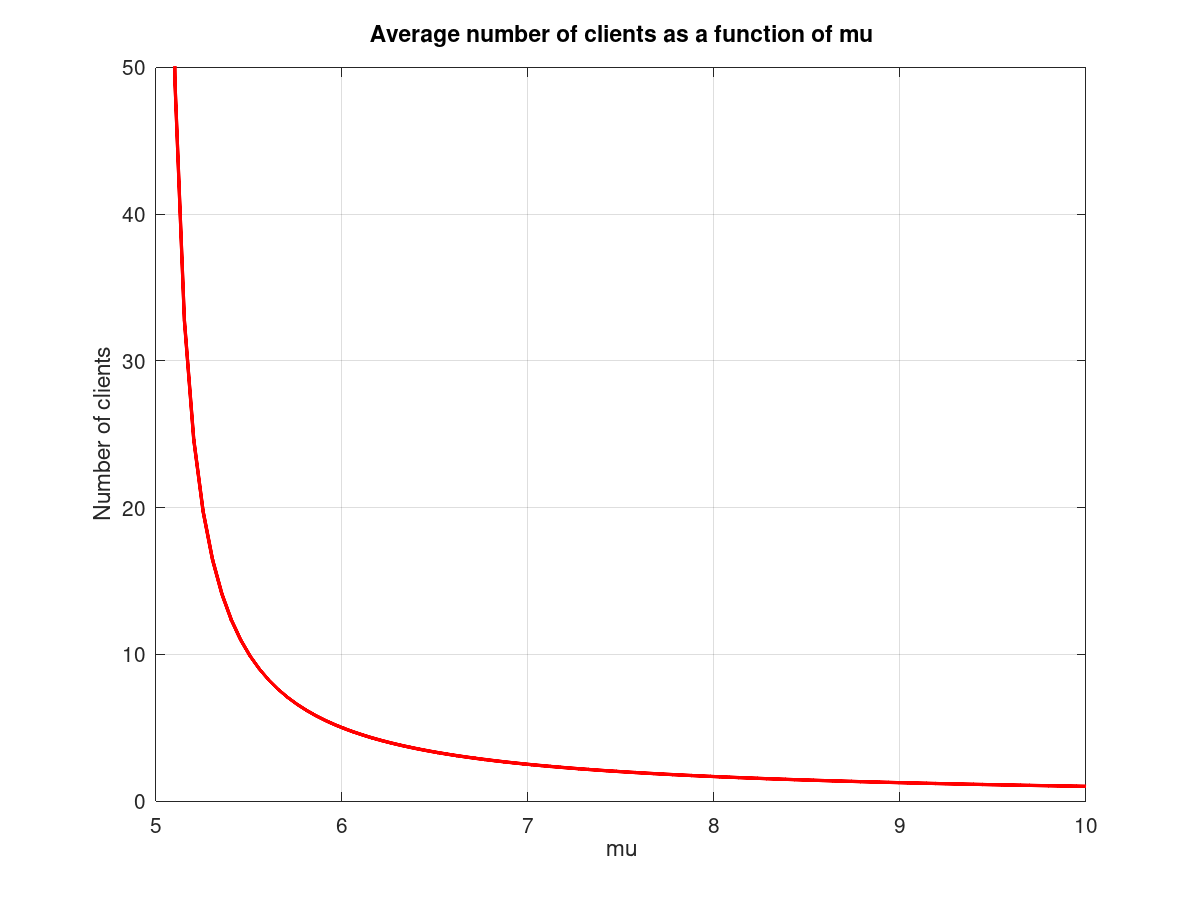
\includegraphics[width=0.85\textwidth]{files/2b3.png}
		\end{center}
	\end{figure}	
	
\end{minipage}
	
\begin{minipage}{\textwidth}
	4. Ρυθμαπόδοση (throughput) ως προς το ρυθμό εξυπηρέτησης:
	\[
		γ = λ \left(1-P[blocking]\right) = λ 
	\]
	\begin{figure}[H]
		\begin{center}
			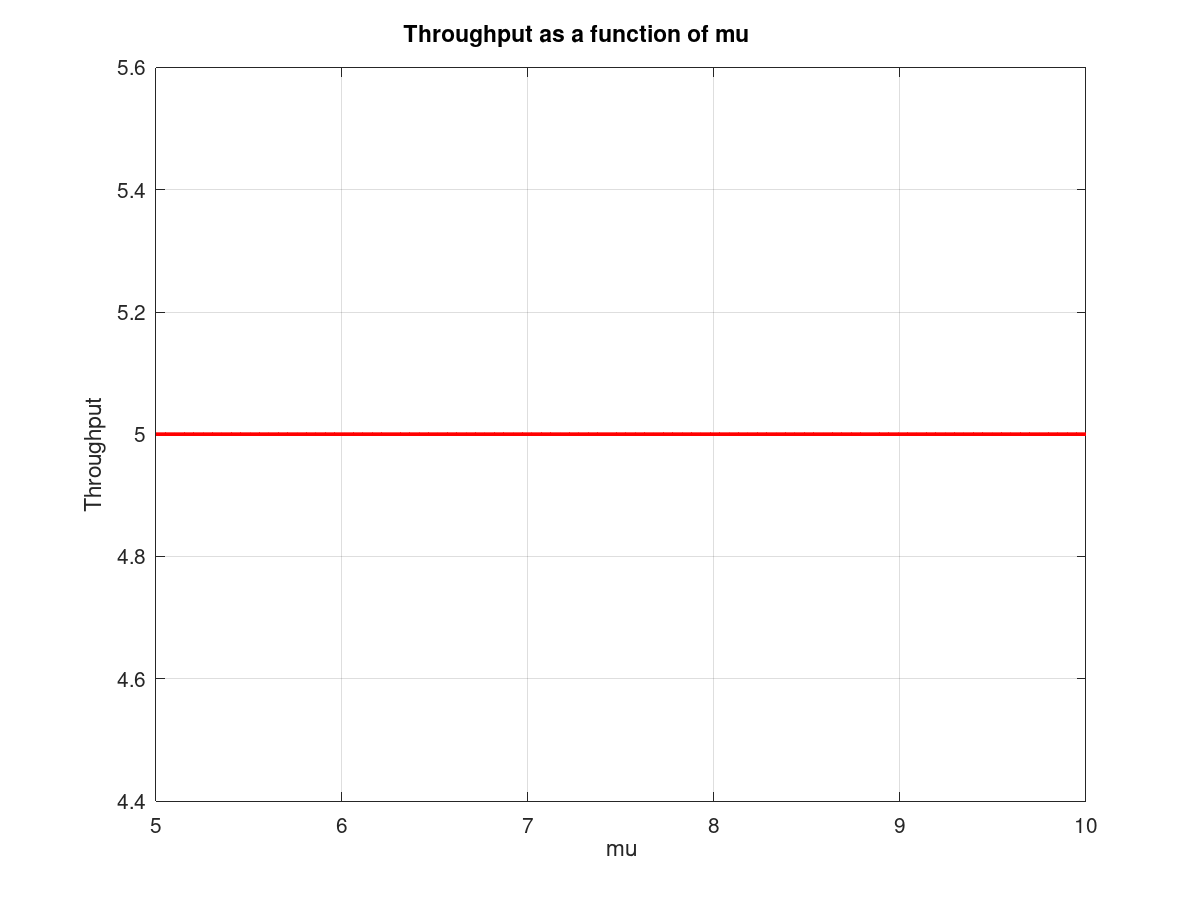
\includegraphics[width=0.85\textwidth]{files/2b4.png}
		\end{center}
	\end{figure}
\end{minipage}

\subsubsection*{(γ)}

Παρατηρώντας το διάγραμμα του μέσου χρόνου καθυστέρησης βλέπουμε, όπως είναι λογικό, ότι όσο αυξάνεται ο ρυθμός εξυπηρέτησης, τόσο ο χρόνος καθυστέρησης μειώνεται. Όμως, η επίδραση που έχει ο ρυθμός εξυπηρέτησης είναι πολύ πιο μεγάλη για τιμές κοντά στο $ μ = 5 $, και μειώνεται όσο το $ μ $ πλησιάζει στο $ 10 $. Έτσι, μπορεί ένας εξυπηρετητής με $ μ = 10 $ να είναι η ιδανική περίπτωση, όμως αν οι απαιτήσεις μας δεν είναι τόσο μεγάλες, αποτελεί σπατάλη πόρων. Για παράδειγμα, πιο λογική επιλογή θα ήταν να διαλέξουμε έναν εξυπηρετητή με $ μ = 6 $, ώστε να αποφύγουμε μεν το κατακόρυφο τμήμα της συνάρτησης-υπερβολής (οπότε επιτυγχάνουμε μέση καθυστέρηση 1 min), αλλά και ταυτόχρονα να μην επιλέξουμε έναν αδικαιολόγητα ακριβό εξυπηρετητή.

\subsubsection*{(δ)}

Παρατηρούμε ότι το throughput πελατών σε μία ουρά Μ/Μ/1 είναι σταθερό και ίσο με $λ$, ανεξάρτητο του $μ$. Αυτό ισχύει διότι, λόγω της άπειρης χωρητικότητας, δεν υπάρχει περίπτωση να απορρίψουμε κανέναν πελάτη, και άρα
\[
	P[blocking] = 0.
\] 
Έτσι, 
\[
	γ = λ (1-P[blocking]) = λ.
\]
\subsection*{Διαδικασία γεννήσεων θανάτων (birth-death process): εφαρμογή σε σύστημα Μ/Μ/1/Κ}

\subsubsection*{(α)}

Μοντελοποιούμε το σύστημα της εκφώνησης ως διαδικασία γεννήσεων-θανάτων.

Το διάγραμμα ρυθμού μεταβάσεων είναι το εξής:

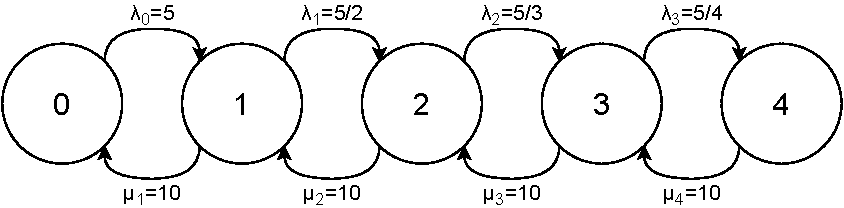
\includegraphics[width=\textwidth]{files/3a.pdf}

Χρησιμοποιώντας τις τοπικές εξισώσεις ισορροπίας έχουμε: 

\begin{align*}
	λ_0P_0=μ_1P_1 &\implies P_1 = \frac{λ_0}{μ_1}P_0 = \frac{P_0}{2} \\
	λ_1P_1=μ_2P_2 &\implies P_2 = \frac{λ_1}{μ_2}P_1 = \frac{P_0}{8} \\
	λ_2P_2=μ_3P_3 &\implies P_3 = \frac{λ_2}{μ_3}P_2 = \frac{P_0}{48} \\
	λ_3P_3=μ_4P_4 &\implies P_4 = \frac{λ_3}{μ_4}P_3 = \frac{P_0}{384} \\
	P_0+P_1+P_2+P_3+P_4=1 &\implies P_0 = \frac{1}{1+1/2+1/8+1/48+1/384}
\end{align*}

οπότε:
\[
	P_0 = 60.66\%, P_1 = 30.33\%, P_2 = 7.58\%, P_3 = 1.26\%, P_4 = 0.16\%
\]

και έτσι: 
\[
	P[blocking] = P_4 = 0.16\%
\]

\subsubsection*{(β)}

\paragraph{(i)}

Η μήτρα ρυθμού μεταβάσεων είναι η εξής:

\begin{minipage}{\textwidth}
\verbatiminput{files/3bi.txt}
\end{minipage}

\paragraph{(ii)}

Με την εντολή ctmc βρίσκουμε τις εργοδικές πιθανότητες των καταστάσεων του συστήματος:

\verbatiminput{files/3bii.txt}

Οι παραπάνω πιθανότητες συμφωνούν με τους θεωρητικούς υπολογισμούς του ερωτήματος (α).

\begin{figure}[H]
	\begin{center}
		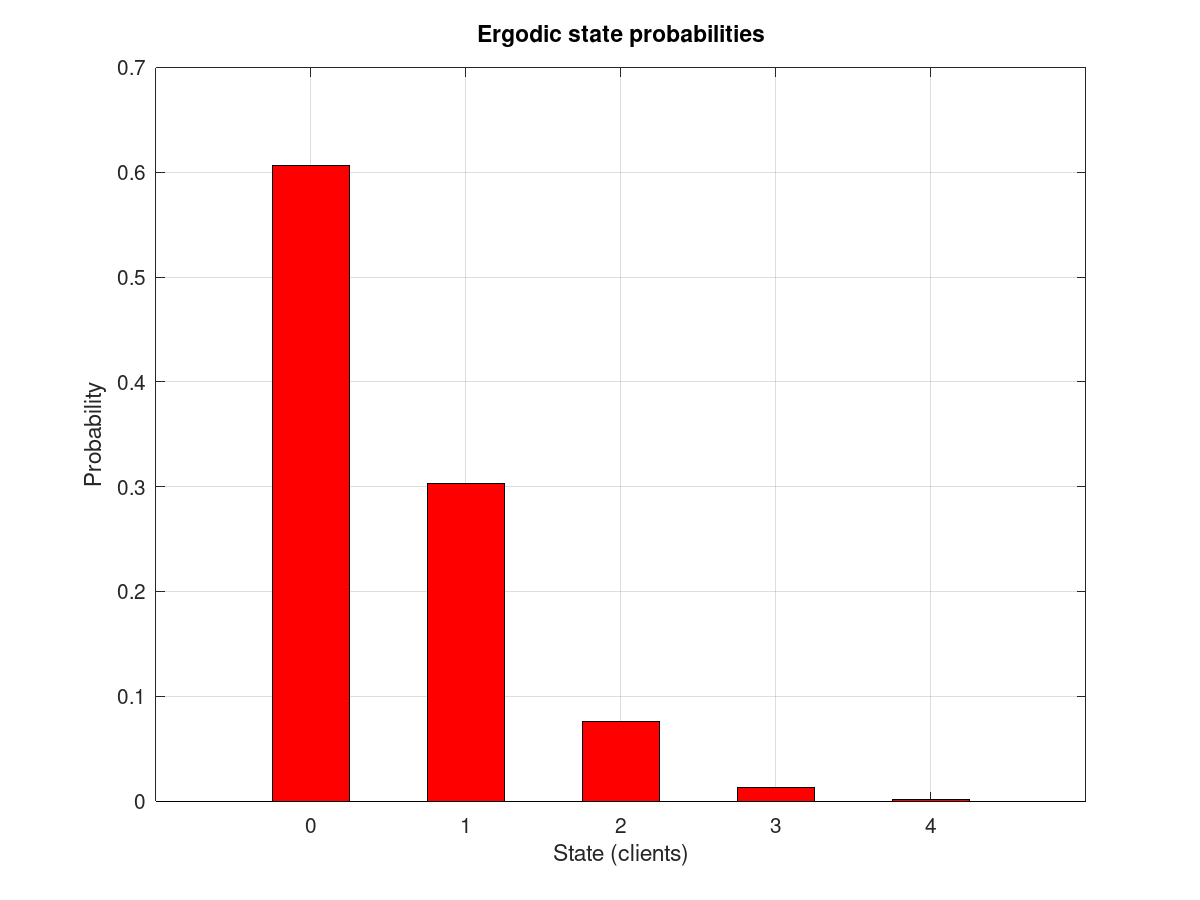
\includegraphics[width=\textwidth]{files/3bii.png}
	\end{center}
\end{figure}

\paragraph{(iii)}

Ο μέσος αριθμός πελατών στο σύστημα όταν αυτό βρίσκεται σε κατάσταση ισορροπίας υπολογίζεται από τη σχέση 
\[
	\sum_{k=0}^5 kP_k 
\]

Ο παραπάνω τύπος δίνει: 

\verbatiminput{files/3biii.txt}

\paragraph{(iv)}

Η πιθανότητα απόρριψης πελάτη όταν το σύστημα βρίσκεται σε κατάσταση ισορροπίας είναι ίση με την πιθανότητα της τελευταίας κατάστασης, δηλαδή την $ P_4 $. Έτσι:

\verbatiminput{files/3biv.txt}

\paragraph{(v)}

Δημιουργούμε τα ζητούμενα διαγράμματα, τα οποία απεικονίζουν την εξέλιξη των πιθανοτήτων για κάθε κατάσταση συναρτήσει του χρόνου, από την αρχική κατάσταση μέχρι οι πιθανότητες να απέχουν λιγότερο από 1\% σε σχέση με τις εργοδικές πιθανότητες του ερωτήματος (2):

\begin{figure}[H]
	\begin{center}
		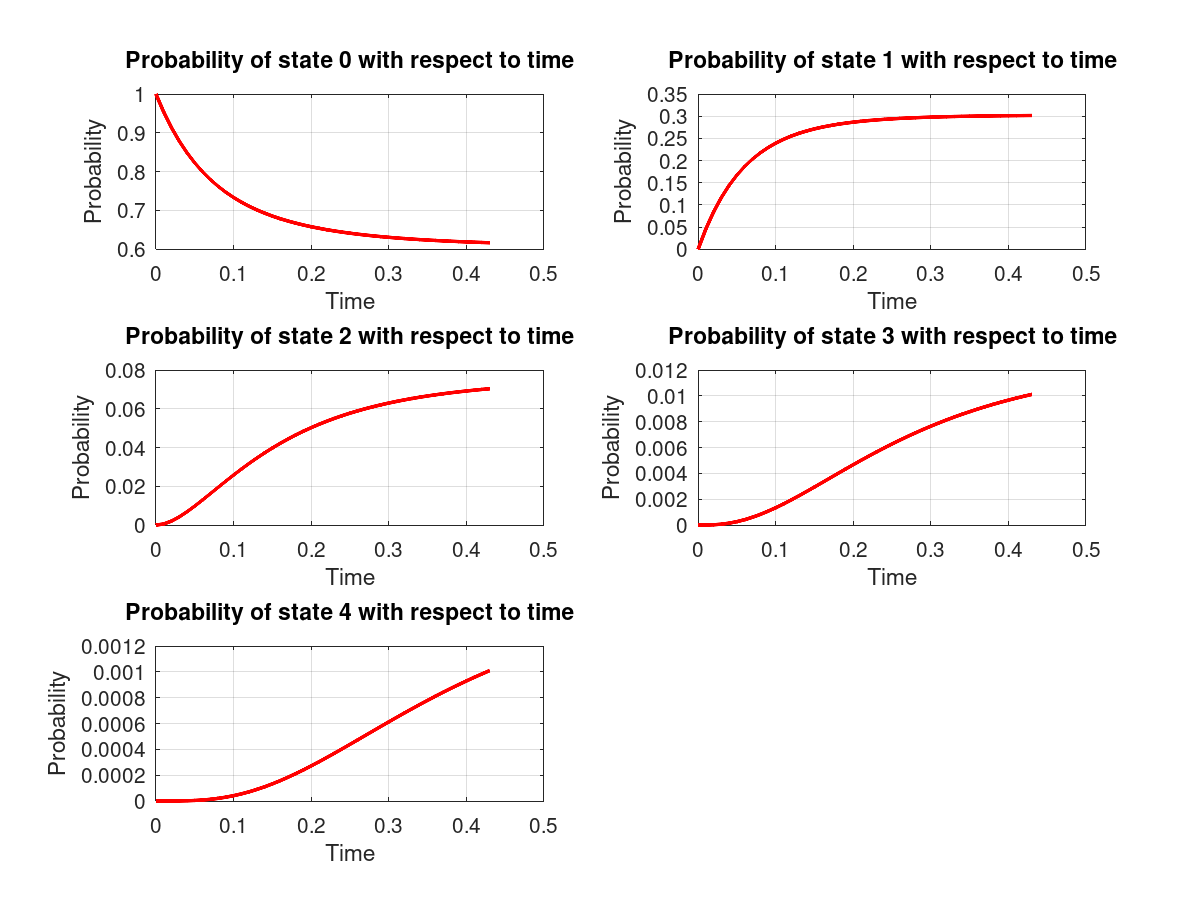
\includegraphics[width=\textwidth]{files/3bv.png}
	\end{center}
\end{figure}


\begin{minipage}{\textwidth}
\paragraph{(vi)}

Επαναλαμβάνουμε για:

	
	\begin{figure}[H]
		1. λ = 5, μ = 1 
		\begin{center}	
			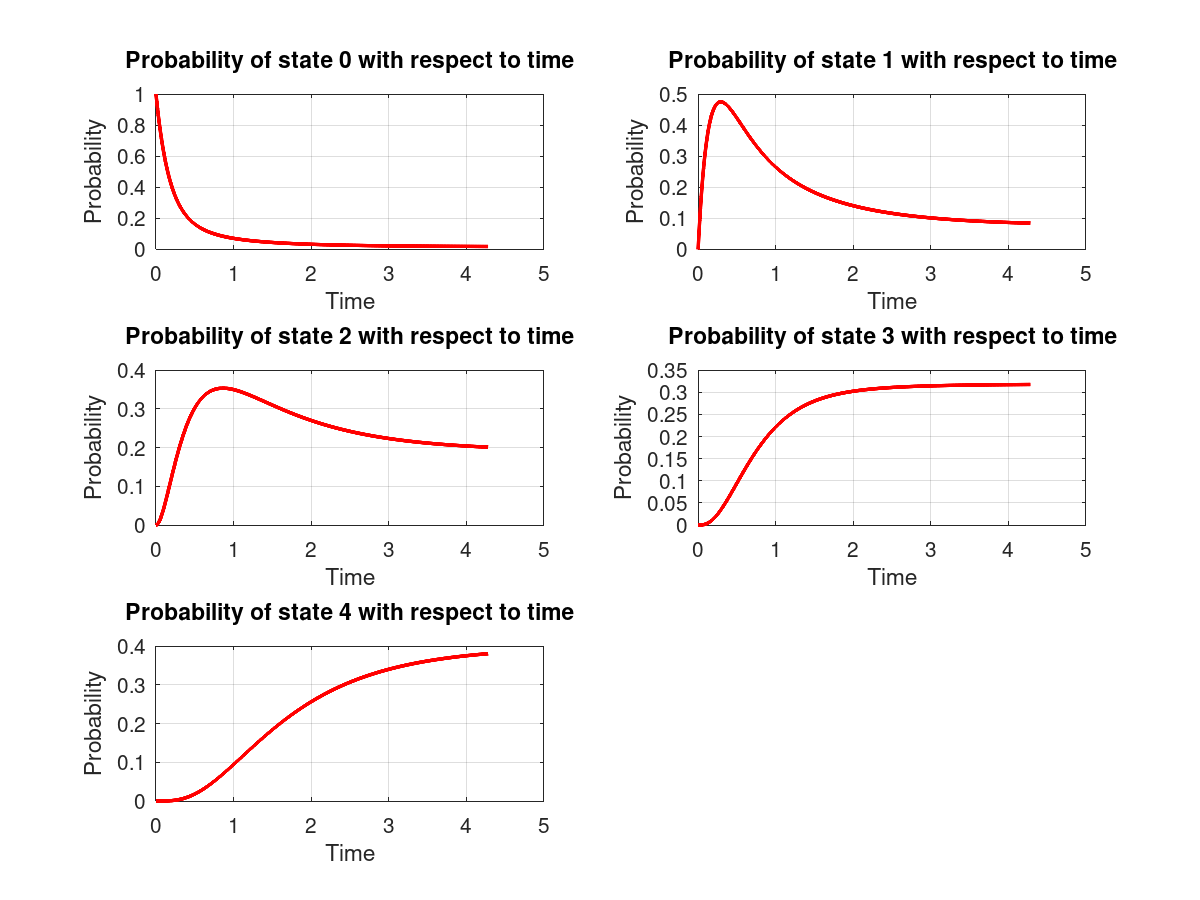
\includegraphics[width=\textwidth]{files/3bvi_1.png}
		\end{center}
	\end{figure}

	
	\begin{figure}[H]
	2. λ = 5, μ = 5
		\begin{center}
			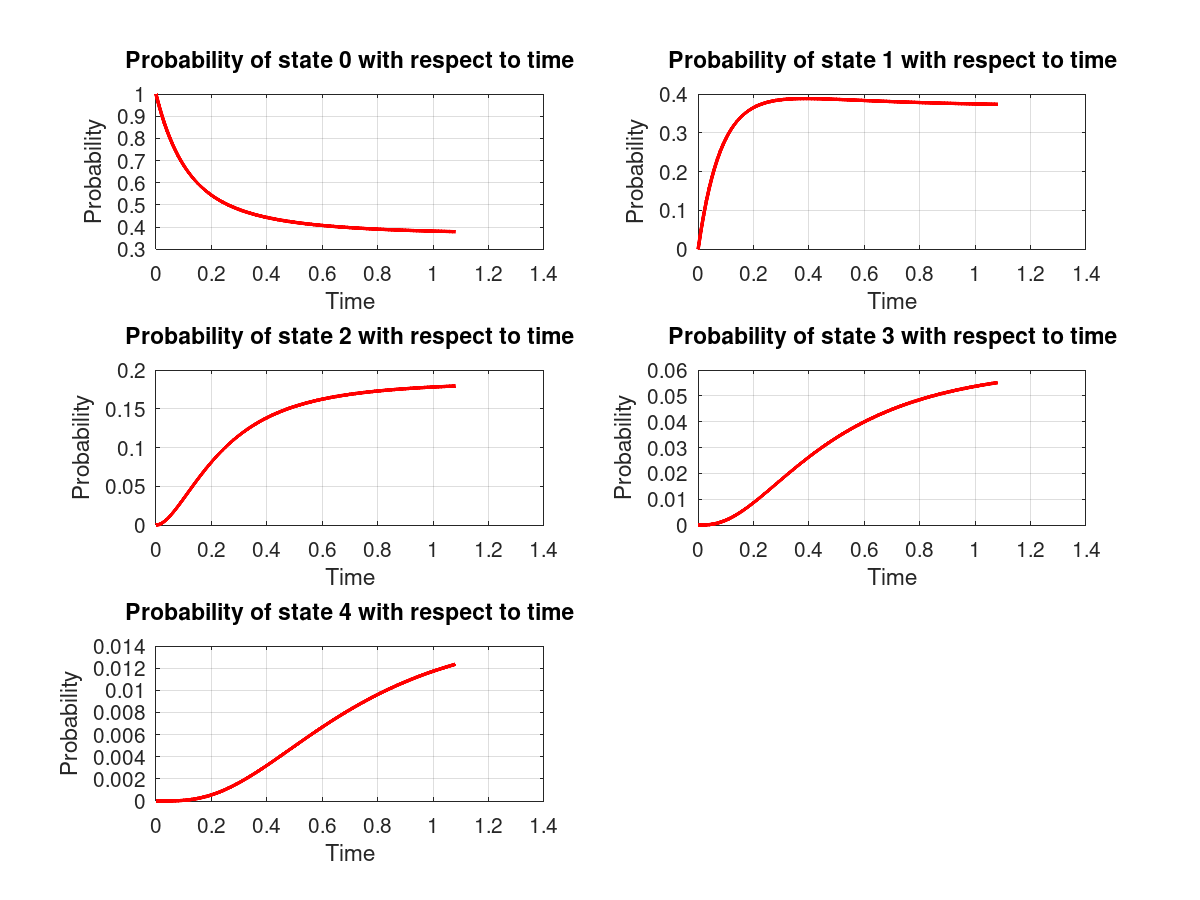
\includegraphics[width=\textwidth]{files/3bvi_2.png}
		\end{center}
	\end{figure}
\end{minipage}
	
	
	\begin{figure}[H]
	3. λ = 5, μ = 20
		\begin{center}
			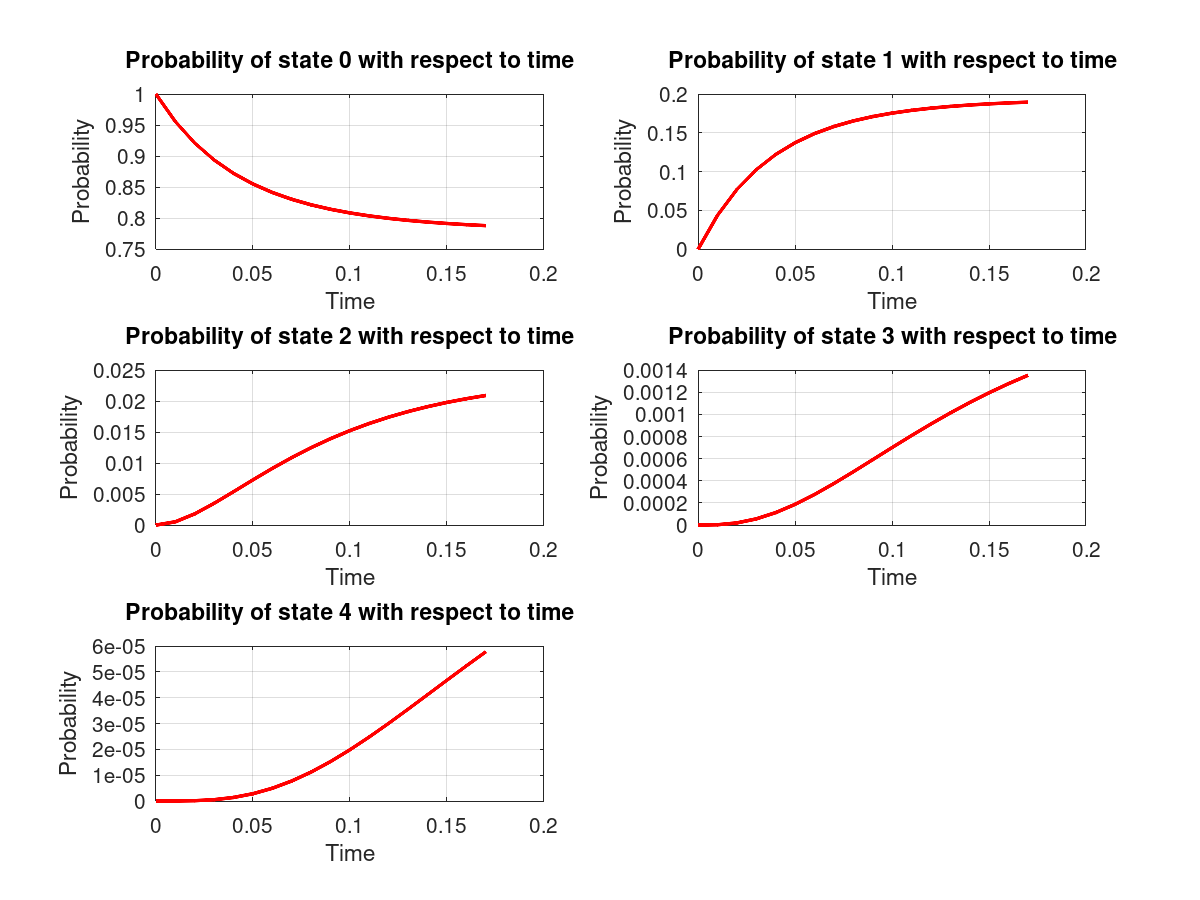
\includegraphics[width=\textwidth]{files/3bvi_3.png}
		\end{center}
	\end{figure}
	
	Ποιοτικά, παρατηρούμε ότι όσο μεγαλώνει η τιμή της παραμέτρου $ μ $:
	\begin{itemize}
		\item Οι πιθανότητες συγκλίνουν γρηγορότερα στις αντίστοιχες εργοδικές.
		\item Οι καταστάσεις με λιγότερους πελάτες έχουν όλο και μεγαλύτερη πιθανότητα να συμβούν. Αυτό συμβαίνει διότι οι πελάτες, οι οποίοι σε όλες τις περιπτώσεις έρχονται με σταθερό ρυθμό, εξυπηρετούνται γρηγορότερα, οπότε το σύστημα αδειάζει συχνότερα. 
	\end{itemize}
	
\subsection*{Παράρτημα κώδικα}

\subsubsection*{Ανάλυση ουράς Μ/Μ/1 με Octave}

\lstinputlisting[language=Octave]{mm1.m}

\subsubsection*{Διαδικασία γεννήσεων θανάτων: εφαρμογή σε σύστημα Μ/Μ/1/Κ}

\lstinputlisting[language=Octave]{mm1k.m}	
\end{document}
